% a0poster Portrait Poster
% LaTeX Template
% Version 1.0 (22/06/13)
%
% The a0poster class was created by:
% Gerlinde Kettl and Matthias Weiser (tex@kettl.de)
%
% This template has been downloaded from:
% http://www.LaTeXTemplates.com
%
% License:
% CC BY-NC-SA 3.0 (http://creativecommons.org/licenses/by-nc-sa/3.0/)
%

%----------------------------------------------------------------------------------------
%	PACKAGES AND OTHER DOCUMENT CONFIGURATIONS
%----------------------------------------------------------------------------------------

% \directlua{pdf.setminorversion(7)}
\documentclass[a0,portrait]{a0poster}

\usepackage{multicol} % This is so we can have multiple columns of text side-by-side
\columnsep=100pt % This is the amount of white space between the columns in the poster
% \columnseprule=3pt % This is the thickness of the black line between the columns in the poster

\usepackage[svgnames]{xcolor} % Specify colors by their 'svgnames', for a full list of all colors available see here: http://www.latextemplates.com/svgnames-colors

\usepackage{times} % Use the times font
%\usepackage{palatino} % Uncomment to use the Palatino font

\usepackage{graphicx} % Required for including images
\graphicspath{{figures/}} % Location of the graphics files
\usepackage{booktabs} % Top and bottom rules for table
\usepackage[font=small,labelfont=bf]{caption} % Required for specifying captions to tables and figures
\usepackage{amsfonts, amsmath, amsthm, amssymb} % For math fonts, symbols and environments
\usepackage[english]{babel}
\usepackage[T1]{fontenc}
\usepackage[utf8]{inputenc}
\usepackage{wrapfig} % Allows wrapping text around tables and figures
\usepackage{bm}
\usepackage{tikz}
\usepackage[skins]{tcolorbox}
\usepackage[hidelinks]{hyperref}

% Shrink bottom margin
\addtolength{\textheight}{7cm}
\begin{document}
%
%----------------------------------------------------------------------------------------
%	POSTER HEADER
%----------------------------------------------------------------------------------------
%
% The header is divided into two boxes:
% The first is 75% wide and houses the title, subtitle, names, university/organization and contact information
% The second is 25% wide and houses a logo for your university/organization or a photo of you
% The widths of these boxes can be easily edited to accommodate your content as you see fit
%
% \begin{minipage}[b]{0.75\linewidth}
\begin{minipage}[b]{0.6\linewidth}
 \VERYHuge \color{Black} \textbf{pyhf} \color{Black}\\[0.5cm] % Title
 \Huge{pure Python implementation of HistFactory}\\[1cm] % Subtitle
 % \author{{\href{https://www.matthewfeickert.com/}{\underline{Matthew Feickert}$^{1}$}}, \href{http://www.lukasheinrich.com/}{Lukas Heinrich$^{2}$}, \href{https://giordonstark.com/}{Giordon Stark$^{3}$}, \href{http://theoryandpractice.org/}{Kyle Cranmer$^{4}$}}
 % \institution{1 Southern Methodist University,~~~2 CERN,~~~3 University of California Santa Cruz,~~~4 New York University}
 \color{DarkSlateGray} % DarkSlateGray color for the rest of the content
 \LARGE {\href{https://www.matthewfeickert.com/}{\underline{Matthew Feickert}$^{1}$}}, \href{http://www.lukasheinrich.com/}{Lukas Heinrich$^{2}$}, \href{https://giordonstark.com/}{Giordon Stark$^{3}$}, \href{http://theoryandpractice.org/}{Kyle Cranmer$^{4}$}\\[0.5cm] % Author(s)
 \normalsize {1 University of Illinois at Urbana-Champaign,~2 CERN,~3 University of California Santa Cruz,~4 New York University}\\[1cm]% University/organization
 % \LARGE\color{MediumBlue} \texttt{john@LaTeXTemplates.com} --- 1 (000) 111 1111\\
 \color{Black}
 \begin{minipage}{0.2\linewidth}
  \begin{center}
   \href{https://pypi.org/project/pyhf/}{
\includegraphics[width=\linewidth]{pyhf_PyPI.pdf}}
  \end{center}
 \end{minipage}%
 \quad
 \begin{minipage}{0.3\linewidth}
  \begin{center}
   \href{https://doi.org/10.5281/zenodo.1169739}{
\includegraphics[width=\linewidth]{zenodo_doi.pdf}}
  \end{center}
 \end{minipage}%
\end{minipage}
%
\begin{minipage}[t]{0.15\linewidth}
 \begin{center}
  \begin{tikzpicture}
   \node[circle,draw,inner sep=2.5cm,fill overzoom image=collaborators/feickert.jpg] (A) {};
  \end{tikzpicture}
 \end{center}
\end{minipage}
\begin{minipage}[b]{0.25\linewidth}
 % 
\includegraphics[width=20cm]{pyhf-logo.png}\\
 
\includegraphics[width=\linewidth]{pyhf-logo.png}\\
\end{minipage}

\vspace{1cm} % A bit of extra whitespace between the header and poster content

%----------------------------------------------------------------------------------------

\begin{multicols}{2} % This is how many columns your poster will be broken into, a portrait poster is generally split into 2 columns

 %----------------------------------------------------------------------------------------
 %	ABSTRACT
 %----------------------------------------------------------------------------------------

 % \color{Navy} % Navy color for the abstract

 %----------------------------------------------------------------------------------------
 %	INTRODUCTION
 %----------------------------------------------------------------------------------------

 % \color{SaddleBrown} % SaddleBrown color for the introduction

 \section*{\LARGE\color{MediumBlue} HistFactory}
 \large
 One of the most widely used statistical models in \textbf{high energy physics} for binned measurements and searches

 \begin{center}
  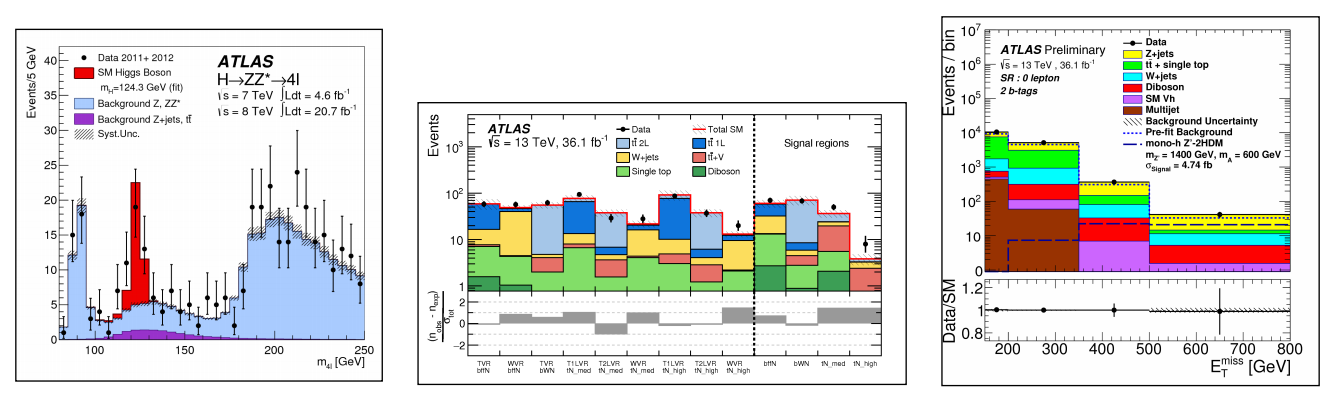
\includegraphics[width=\linewidth]{HistFactory_result_examples.png}
 \end{center}
 %
 \begin{minipage}{0.33\linewidth}
  \begin{flushleft}
   \large\quad~~\textbf{Standard Model}
  \end{flushleft}
 \end{minipage}%
 \quad
 \begin{minipage}{0.33\linewidth}
  \begin{flushleft}
   \large\quad~\textbf{Supersymmetry}
  \end{flushleft}
 \end{minipage}%
 \quad
 \begin{minipage}{0.33\linewidth}
  \begin{flushleft}
   \large\qquad~~\textbf{Exotics}
  \end{flushleft}
 \end{minipage}%

 \section*{\LARGE\color{MediumBlue} Declarative binned likelihoods}

 \[
  f(\bm{n}, \bm{a} \,|\,\bm{\phi},\bm{\chi}) = \underbrace{\color{blue}{\prod_{c\in\mathrm{\,channels}} \prod_{b \in \mathrm{\,bins}_c}\textrm{Pois}\left(n_{cb} \,\middle|\, \nu_{cb}\left(\bm{\eta},\bm{\chi}\right)\right)}}_{\substack{\text{Simultaneous measurement}\\%
    \text{of multiple channels}}} \underbrace{\color{red}{\prod_{\chi \in \bm{\chi}} c_{\chi}(a_{\chi} |\, \chi)}}_{\substack{\text{constraint terms}\\%
    \text{for }\text{``auxiliary measurements''}}}
 \]

 \noindent\textcolor{blue}{Primary Measurement}:
 \begin{itemize}
  \item Multiple disjoint ``channels'' (e.g. event observables) each with multiple bins of data
  \item Example parameter of interest: strength of physics signal, $\mu$
 \end{itemize}
 \textcolor{red}{Auxiliary Measurements}:
 \begin{itemize}
  \item Nuisance parameters (e.g. in-situ measurements of background samples)
  \item Systematic uncertainties (e.g. normalization, shape, luminosity)
 \end{itemize}

 \section*{\LARGE\color{MediumBlue} Performance}
 Efficient use of tensor computation makes pyhf fast
 \begin{center}
  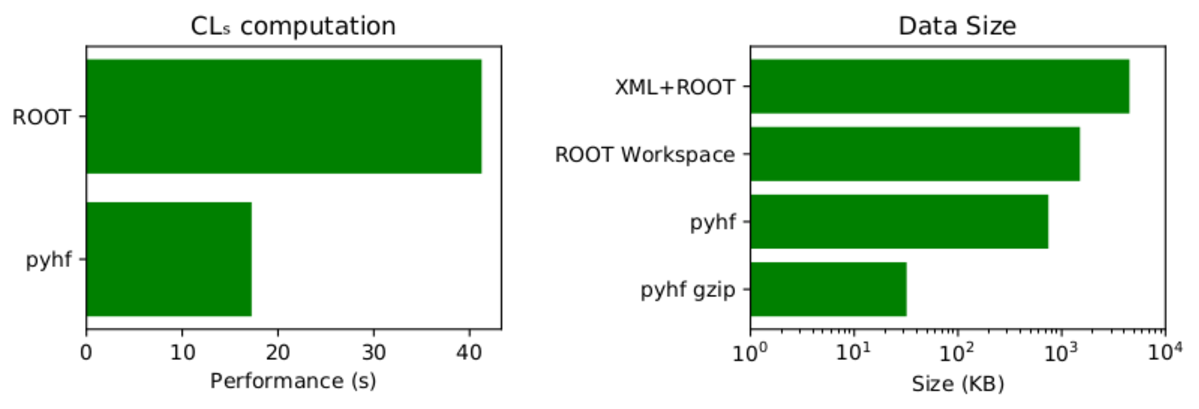
\includegraphics[width=0.9\linewidth]{performance_only.pdf}
 \end{center}
 Competitive with traditional \texttt{C++} implementation --- often faster

 \section*{\LARGE\color{MediumBlue} Hardware Acceleration}
 For machine-learning-library tensor backends the computational graph can be transparently placed on hardware accelerators: \textbf{GPUs} and \textbf{TPUs} for order of magnitude speed-up in computation
 \begin{center}
  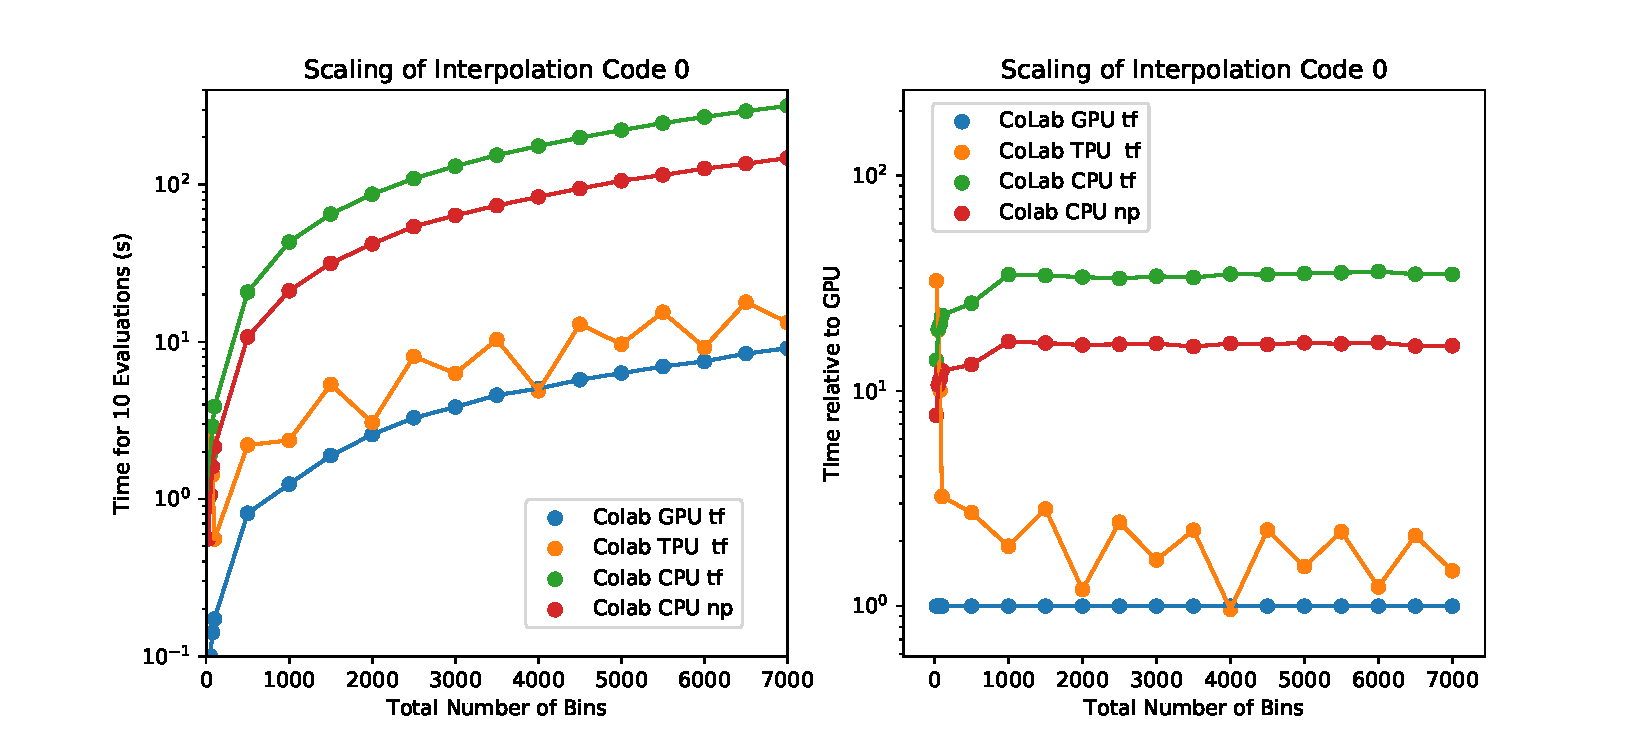
\includegraphics[width=\linewidth]{scaling_hardware.pdf}
 \end{center}

 \section*{\LARGE\color{MediumBlue} Automatic Differentiation}

 Tensor libraries from machine learning frameworks provide exact gradients of computational graphs (likelihood). Useful for minimization!

 \section*{\LARGE\color{MediumBlue} Optimizers}

 Support optimizers that implement Newton's method as well as \texttt{scipy.minimize} and MINUIT. More advanced optimizers to come soon!

 \vspace{1cm}
 \begin{minipage}{0.5\linewidth}
  \begin{flushright}
   \href{https://github.com/diana-hep/pyhf}{
\includegraphics[width=0.3\linewidth]{GitHub_logo.png}}
  \end{flushright}
 \end{minipage}%
 \quad
 \begin{minipage}{0.5\linewidth}
  \begin{flushleft}
   \href{https://github.com/diana-hep/pyhf}{\includegraphics[width=0.3\linewidth]{github_qr_code.pdf}}
  \end{flushleft}
 \end{minipage}%

 \section*{\LARGE\color{MediumBlue} Implementation}
 \begin{center}
  % 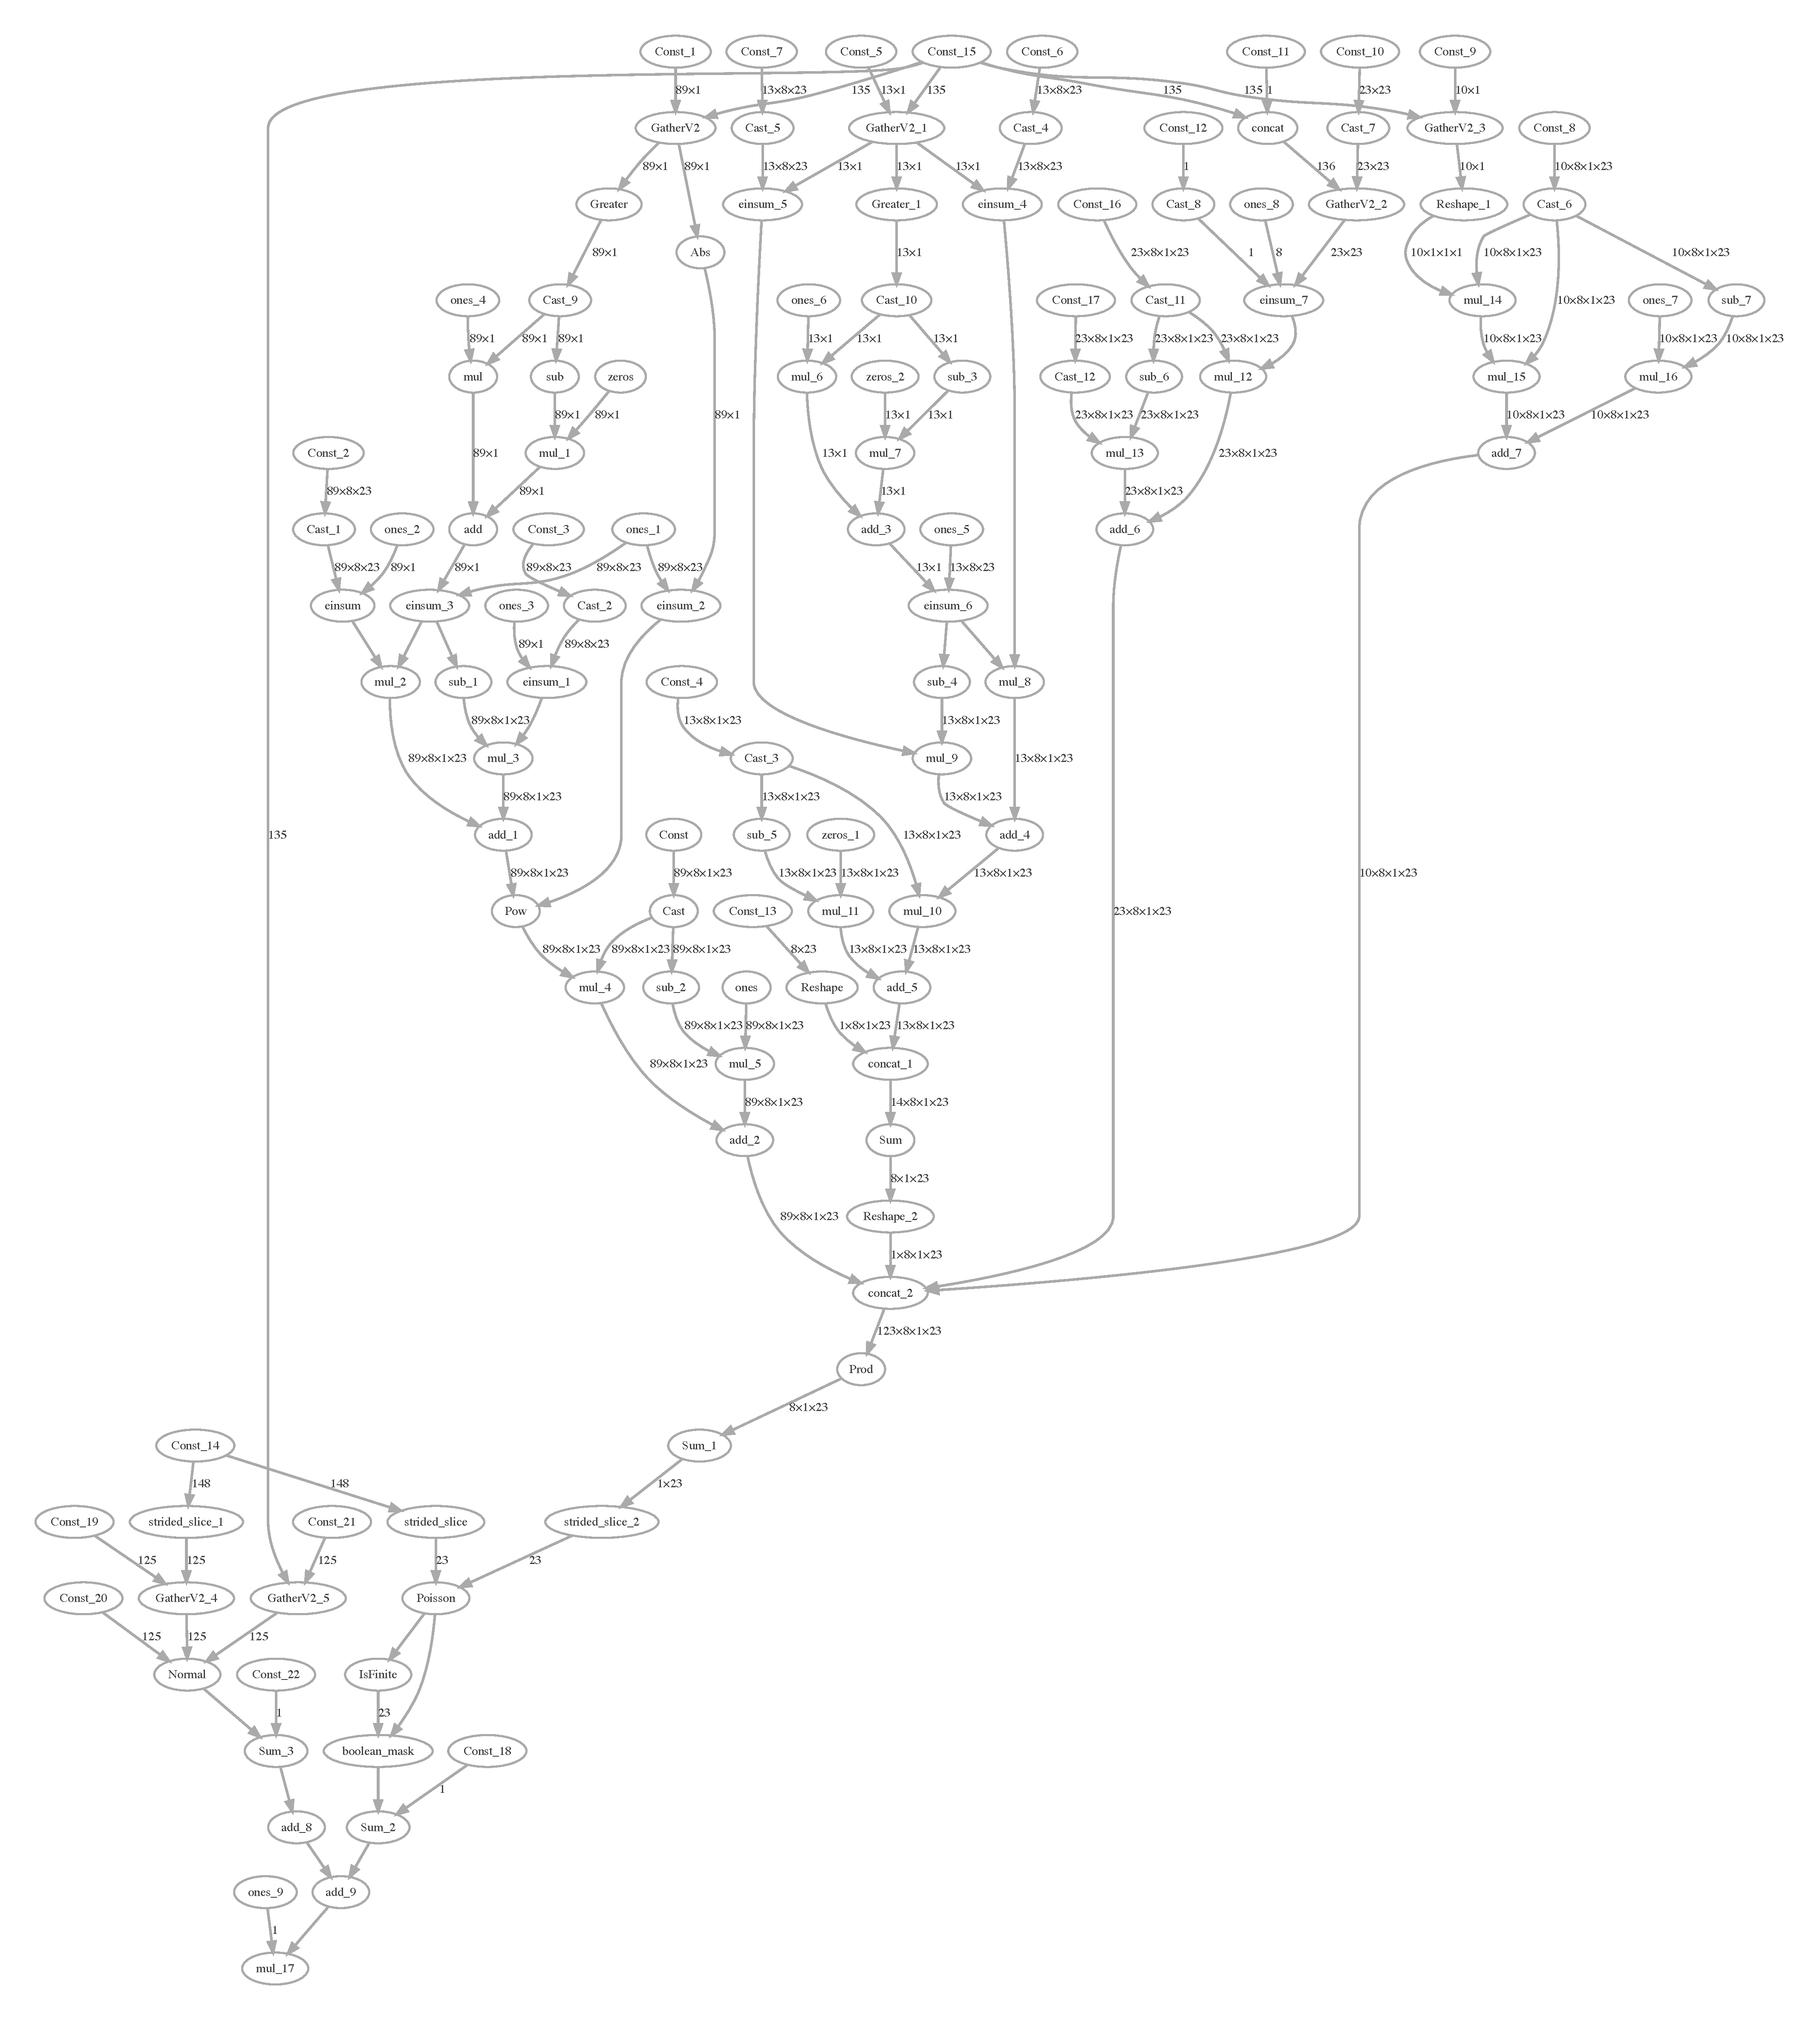
\includegraphics[width=0.8\linewidth]{computational_graph3.pdf}
  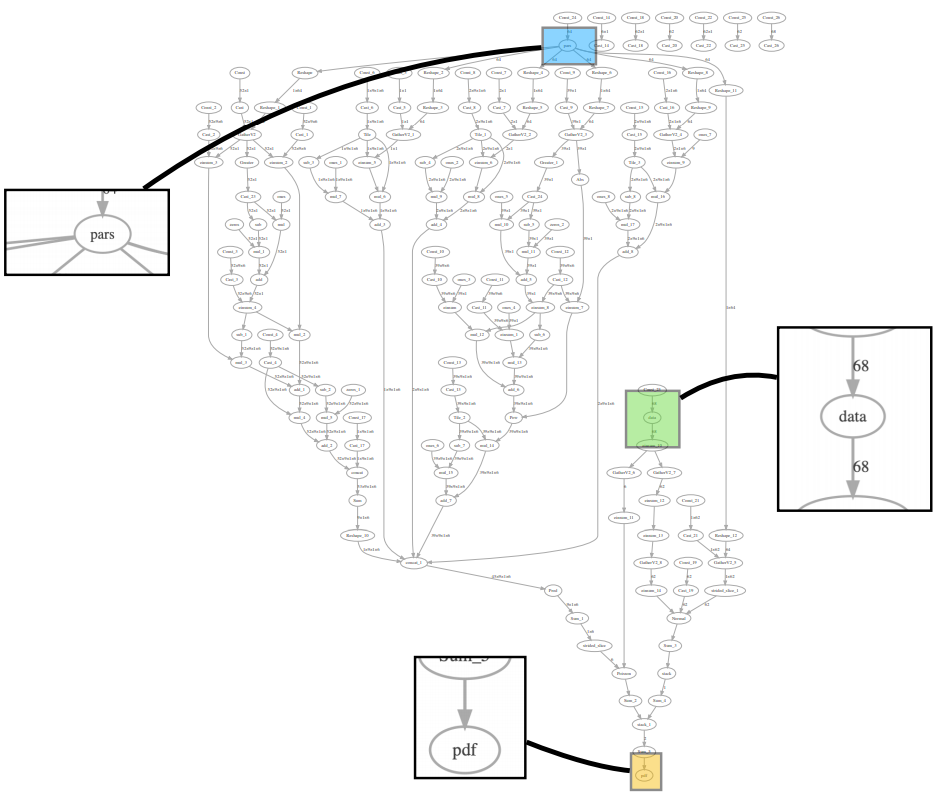
\includegraphics[width=0.9\linewidth]{computational_graph.png}
 \end{center}
 The computational graph of multidimensional array operations for likelihood function of a physics analysis defined through HistFactory

 \vspace{1cm}
 %
 \begin{minipage}{0.33\linewidth}
  \begin{center}
   
\includegraphics[width=\linewidth]{NumPy_logo.pdf}
  \end{center}
 \end{minipage}%
 \quad
 \begin{minipage}{0.33\linewidth}
  \begin{center}
   
\includegraphics[width=\linewidth]{TensorFlow_logo.pdf}
  \end{center}
 \end{minipage}%
 \quad
 \begin{minipage}{0.33\linewidth}
  \begin{center}
   
\includegraphics[width=0.85\linewidth]{Pytorch_logo.pdf}
  \end{center}
 \end{minipage}%
 \vspace{1cm}

 \noindent Use of $n$-dimensional array (``tensor'') operations through a common API layer around high performance tensor libraries


 \section*{\LARGE\color{MediumBlue} JSON Specification}
 The \textcolor{blue}{full likelihood} can be expressed as a \textbf{single JSON document}.\\Archive friendly for analysis presentation! Used by ATLAS to \textcolor{blue}{publish likelihoods} to HEPData (\textcolor{blue}{\href{https://atlas.web.cern.ch/Atlas/GROUPS/PHYSICS/PUBNOTES/ATL-PHYS-PUB-2019-029/}{ATL-PHYS-PUB-2019-029}}).
 \vspace{0.5em}
 \begin{center}
  \href{https://raw.githubusercontent.com/diana-hep/pyhf/master/examples/2-bin_1-channel.json}{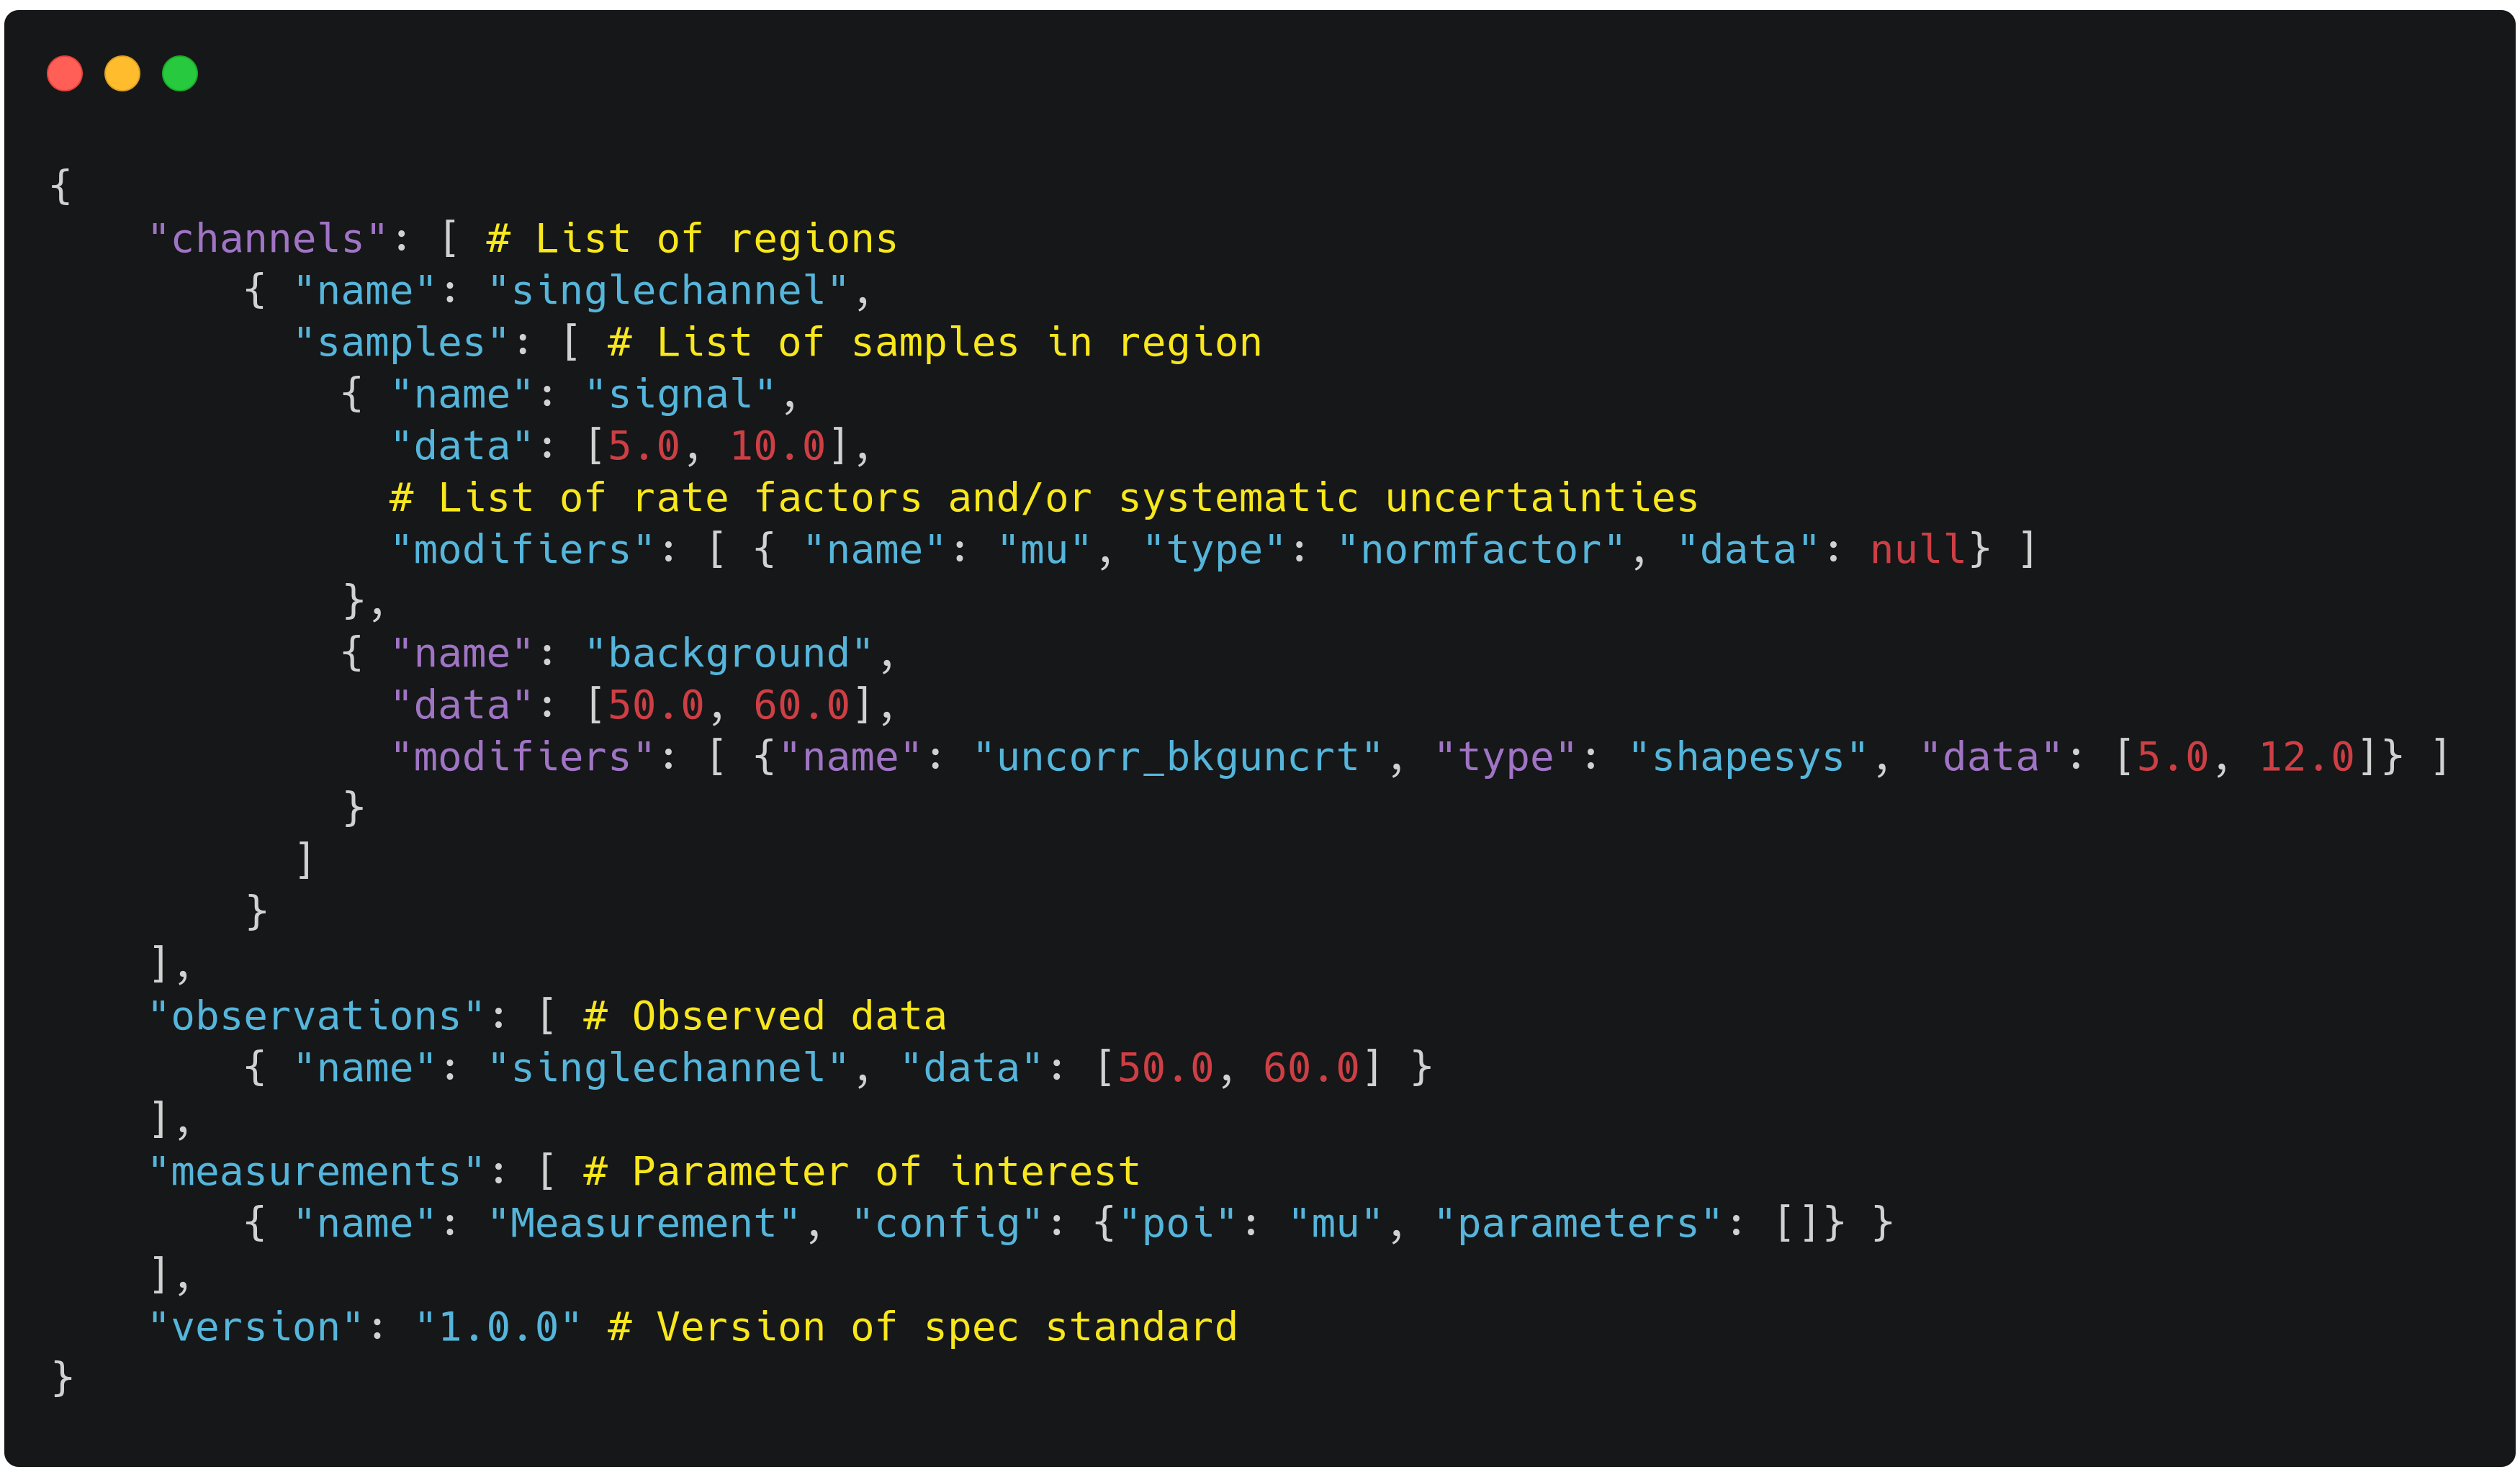
\includegraphics[width=0.7\linewidth]{carbon_JSON_spec_annotated.png}}
 \end{center}
 \vspace{-1em}
 \begin{center}
  {\small\textbf{Example:} 2 binned single channel with 2 samples with 1 parameter of interest and 1 nuisance parameter}
 \end{center}
 \begin{center}
  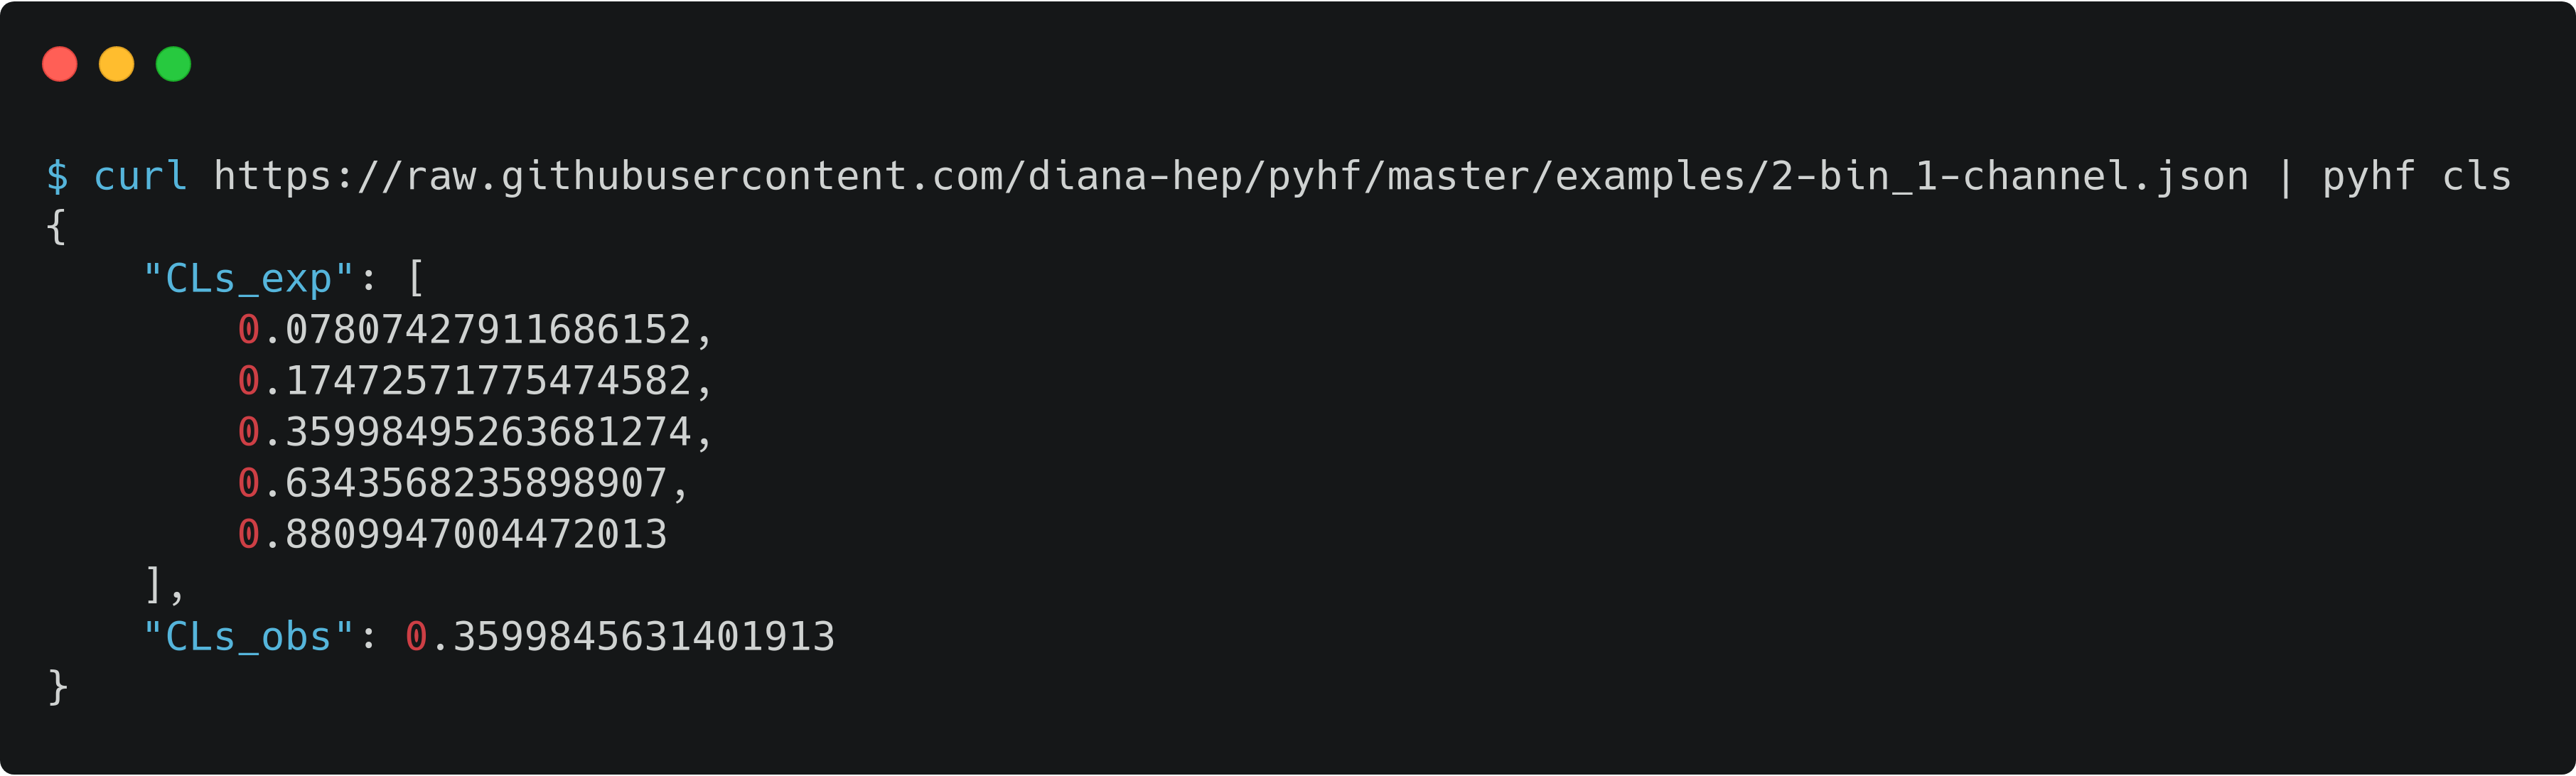
\includegraphics[width=0.7\linewidth]{carbon_pyhf_CLs.png}
 \end{center}

 \begin{center}
  JSON Patch standard allows for reinterpretation with \textcolor{blue}{new signal models}
 \end{center}
 \begin{center}
  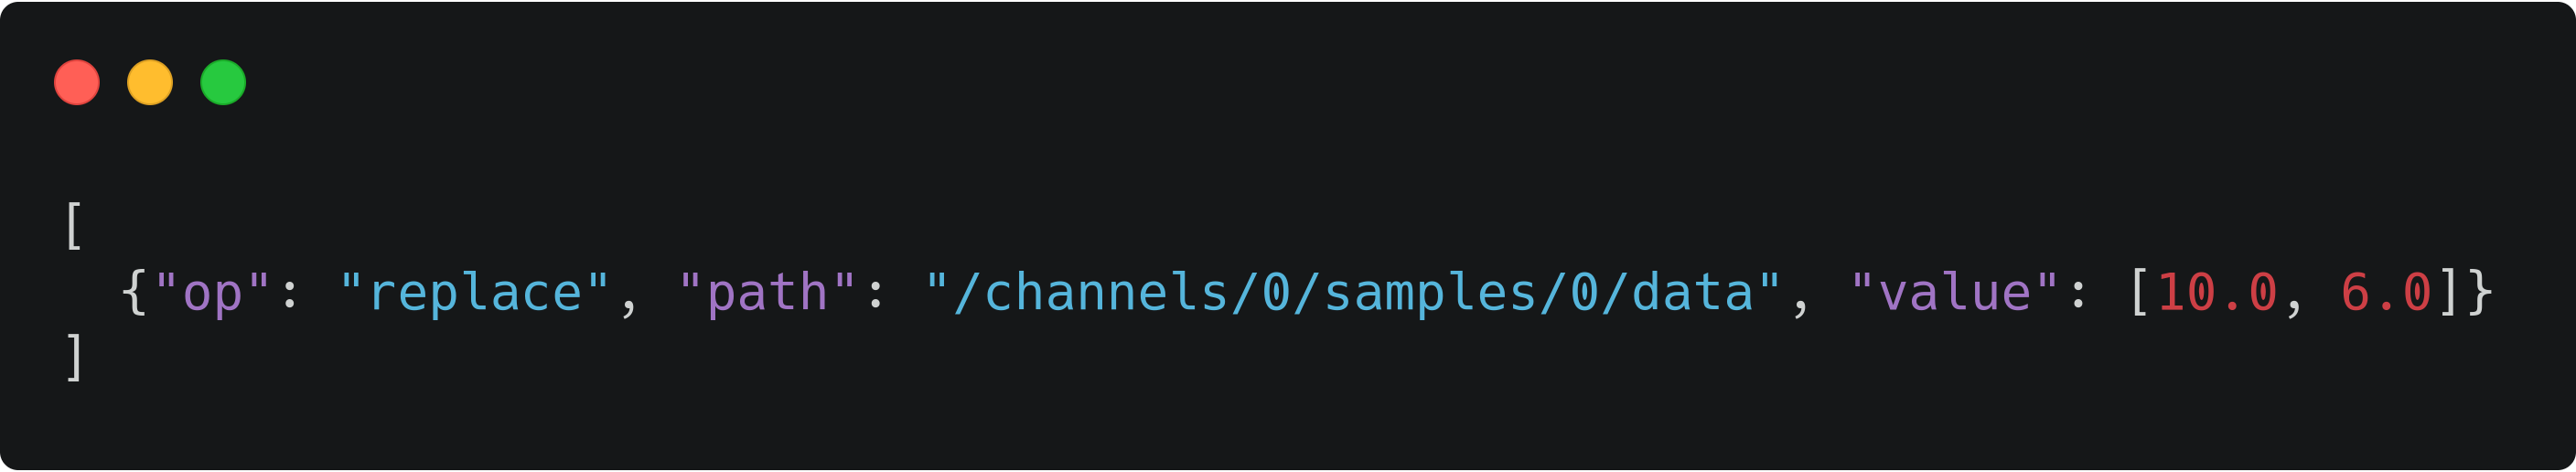
\includegraphics[width=0.7\linewidth]{carbon_JSON_patch.png}
 \end{center}
 %
 \begin{center}
  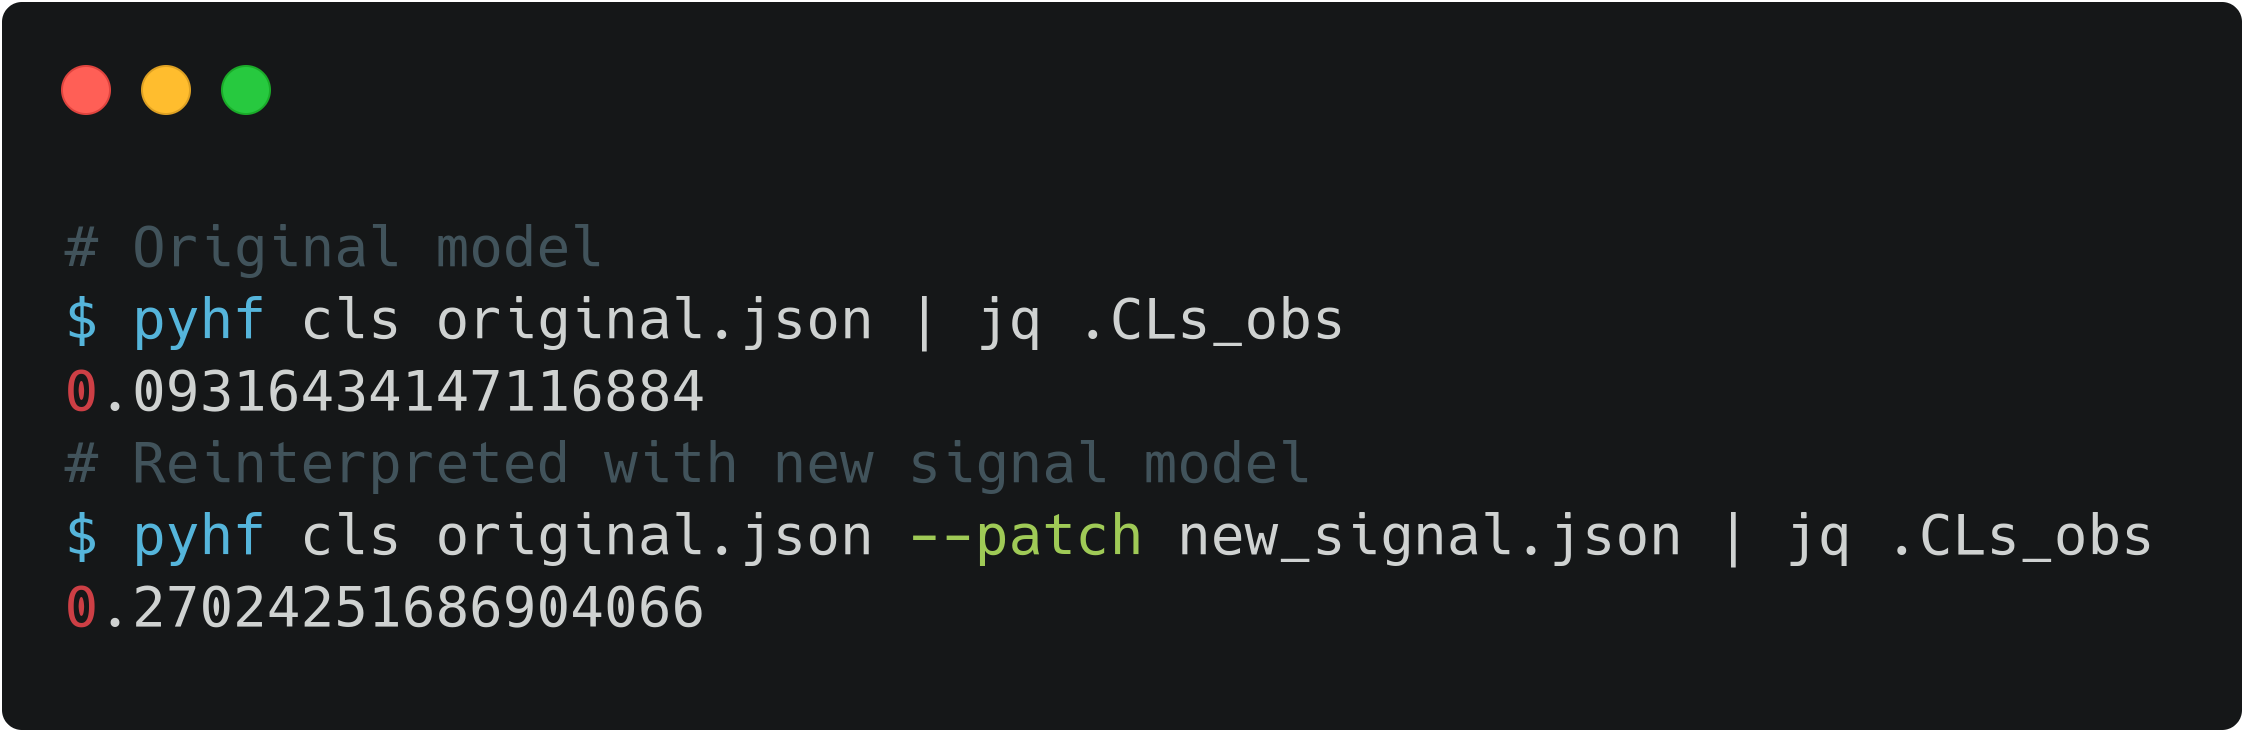
\includegraphics[width=0.7\linewidth]{carbon_reinterpretation.png}
 \end{center}

 \begin{minipage}{0.5\linewidth}
  \begin{flushright}
   \href{https://indico.cern.ch/event/773049/contributions/3476143/}{
    \begin{tikzpicture}
     \node[circle,draw,inner sep=2cm,fill overzoom image=chep2019_logo.png] (A) {};
    \end{tikzpicture}}
  \end{flushright}
 \end{minipage}%
 \quad
 \begin{minipage}{0.5\linewidth}
  \begin{flushleft}
   \href{https://indico.cern.ch/event/773049/contributions/3476143/}{\includegraphics[width=0.3\linewidth]{chep_talk_qr_code.pdf}}
  \end{flushleft}
 \end{minipage}%

\end{multicols}
\end{document}
